\chapter{Approach}
\label{chap:approach}

% TODO add summary of approach
The goal of the research is to provide change prediction. This is accomplished through mining of software data (covered in introduction), analysis of collected data, candidate feature analysis. After the data has been collected it is further analyzed to extract key features. This data is then visualized to provide insights into the data set. Candidate features are then selected from possible features and analyzed to determine the best feature set.
% The complete analysis is done in experiments section

% TODO fix segway into this paragraph

In order to be able to predict changes within a project some project data must first be collected. The data collection is targeted towards open source projects that use GitHub. Specifically projects that are predominately written in Java. The overall method is not language specific however for the purpose of simplifying the implementation it was restricted to only allow for Java. The data collection simply collects all the project's development history realized through the changes made to the project. This includes the information related to developers, commits, tags (releases) and files in the project.

The data is kept unprocessed and stored directly into a relational database (MySQL) which allows the data to be used and manipulated without requiring access to GitHub again. This was ideal during the more initial phase of the research allowing for various methods of analysis to be applied on the dataset without requiring the data to be download again. The collection of data can take long to perform and depends largely on the size of the project. The collection process also allows for a partial collection of newly added project changes after the initial collection of the project. This allows for the changes made to the project after the initial collection of project data to be collected as well. These maintenance collections will often be much smaller and require a smaller amount of time to collect.


%<<< TODO create a table which outlines the data elements >>>
% TODO create a figure of an api return

The method chosen for collecting data for GitHub projects was using GitHub's web \gls{api}. The GitHub \gls{api} allows for access to the complete set of publicly available information stored in GitHub. Accessing the data through the \gls{api} allows for the process to be automated and vastly simplifies the process. This dataset can be rather large since it includes a snapshot of the commit, all the change data and developer data related. In order to collect data the repository name and the name of the user who owns the repository must be known.

To actually collect the data from GitHub a ruby script was used. This collection is built around a Ruby library, \textit{github\_api}, which is a convenient wrapper for GitHub's web \gls{api}. The script systematically collects the desired data related from a given GitHub project to be stored locally. As noted above the collection can take a bit of time to complete since it must go commit by commit to collect the necessary data.

% TODO integrate this with above explanation of VCS and git
Some aspects of the GitHub project's dataset are not collected as they were deemed unnecessary however it could easily be extended to collect the other aspects. The aspects not collected are the issues, branches, forks and pull requests. The issues data outlines the problems reported in the project by users or developers of that project. GitHub allows for issues to be optional and thus some projects do not offer issue reporting through GitHub. Branches are also directly related to the project and they are essentially different workspaces for the developers. They allow for development of different versions (such as a development version compared to a stable version). The simplicities sake this project assumes that the main branch (master) is the development branch and the target of the analysis. Of course other branches could be analyzed however the perspective of the other branches typically originates from the master branch.

A similar sub-data set not collected or used is forks of the repository. For GitHub a fork is an externally created branch. This allows for a developer who does not own the project (but can view it) make a copy of the project and work on it without affecting the original. Forks differ slightly from branches in that they typically denote a deviation from the original project that is unlikely to be reconciled. Finally, pull requests facilitate external developers making small changes which tend to be fixes to problems found or desired feature implementation. The owner of the repository can then decide to integrate the changes made the original repository.


%- TODO explain a little more
%    - about using the api commands and how this is entirely automatic. Simply point to repo owner and name and it collects
%    - language agnostic for collection
%    - What is not collected:
%        - issues
%        - forks
%        - pull requests

\section{Storage}
\label{sec:storage}

As mentioned above the data is stored in a MySQL relational database which leverages \gls{sql}. There are two databases used for the collection and the analysis. One stores the raw mined data, whereas the second stores the analyzed data in a more convenient layout to be used later. A third database stores the same data as the second however it uses relational database implementation because of some limitations within MySQL. This third database uses PostgreSQL, which has some more advanced features than MySQL and is simply a clone of the second database. The specific limitations that were encountered will be discussed more fully later on in this section.

\begin{figure}[!ht]
    \centering
        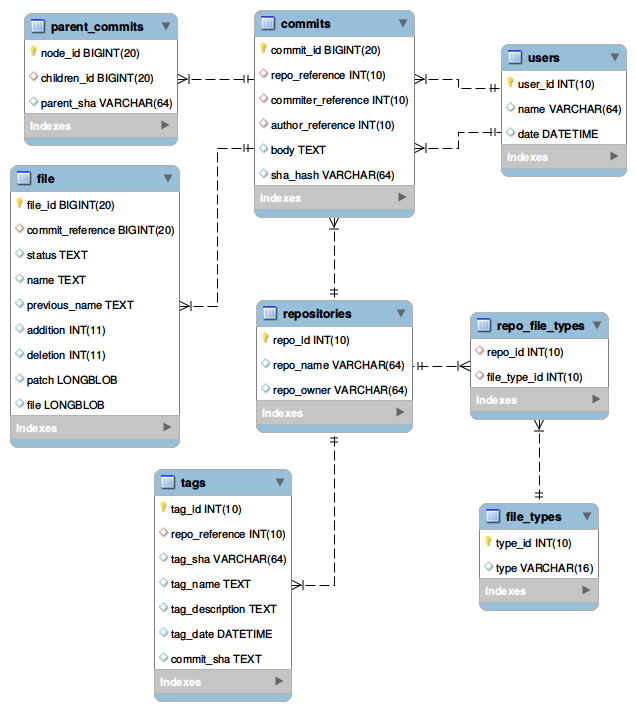
\includegraphics[width=1.0\textwidth]{images/github_data_schema}
    \caption{GitHub Data Schema}
    \label{fig:github_data_schema}
\end{figure}

%TODO re-factor this
The first database called \textit{github\_data} and stores the semi-raw data collected from GitHub's \gls{api}. This database contains 8 tables which store various aspects about the projects that are considered potentially important for the analysis later on. The tables of primary concern are \textit{repositories}, \textit{commits}, \textit{users}, \textit{files} and \textit{tags} tables. The data collection from GitHub's \gls{api} collects primary aspects related to the desired analysis. Other aspects are available from the \gls{api} and if need the database could be extended to store more elements as necessary. In some cases data from the \gls{api} is not available for one reason or another (usually inaccessible files or such) these are simply removed or a note is made of them depending on their importance. For example, files that do not contain Java code are not essential and if inaccessible are ignored. If a Java file is inaccessible a note is made as this is a greater concern. These files can be retrieved if enough information is available (previous version and corresponding patch file). In the case that insufficient information is available the analysis can still be applied but will likely adversely effected the result.

After storing the data in the \textit{github\_data} database, the analysis process is done. The \textit{parsing} script is run next and discussed further in the section \ref{sec:parsing}. This database, \textit{project\_stats}, is very similar in layout to the first database except some extra tables have been added and a few data items have been removed. Mostly the storage expansions have been to hold change information calculated from the analysis of the data.

\begin{figure}[!ht]
    \centering
        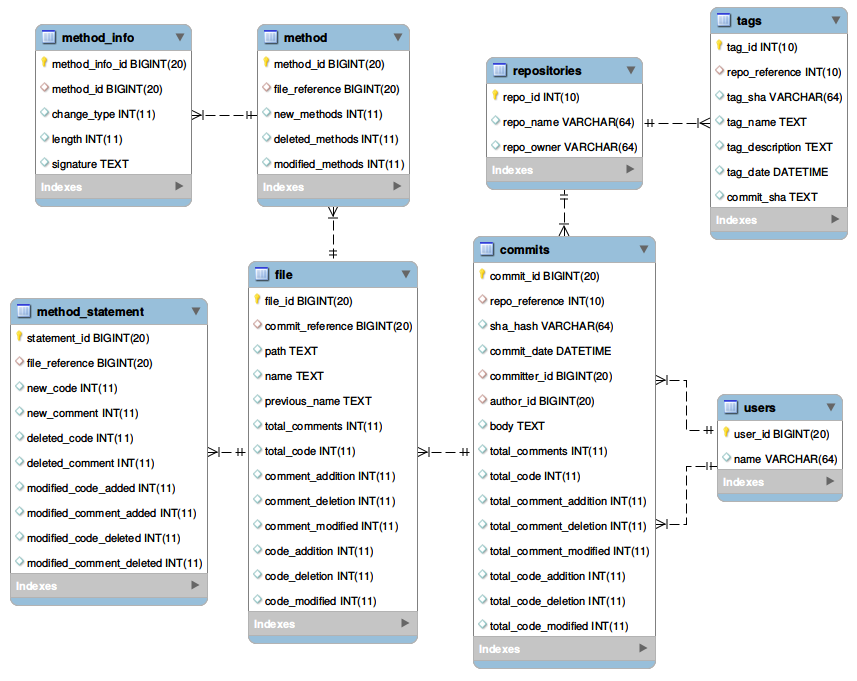
\includegraphics[width=1.0\textwidth]{images/project_stats_schema}
    \caption{Project Stats Schema}
    \label{fig:project_stats_schema}
\end{figure}

The final database uses PostgreSQL because of limitations within the MySQL implementation. Some of the candidate features, discussed in further detail in section \ref{sec:sample_data}, required a more versatile partitioning function and the ability to perform multiple inner queries. The first of which is more difficult to implement and the second is not available at all MySQL.

In order to transfer the data over to PostgreSQL, a simple program called \textit{pgloader}\footnote{\url{http://pgloader.io/}} was used to transfer the MySQL database over to PostgreSQL. Only one difficulty was encountered during the transferring process. One of the tables in the MySQL database was called \textit{user}, however in PostgreSQL this is a reserved table name and therefore the table cannot be interacted with properly. The work around was to simply rename the table in MySQL prior to transferring to avoid any issues with the database. Once the database is copied over to PostgreSQL it is ready to be used for to perform change prediction.

\section{Parsing}
\label{sec:parsing}

When the data has been collected and stored it can then be analyzed to extract more refined details. The changes made per commit can be analyzed to extract the number of methods added, deleted and modified per commit. The process first requires the changes from a commit, the patches, to be merged into their corresponding full file. A patch is simply a summarized stub of the full file which allows for a quick reference as to which line is changed and what change occurred on that line. The three different types of changes that can appear within a file are deletions, additions and no change. These are represented as a minus sign, plus sign and space respective.

% TODO talk about these different changes
% TODO consider getting different images (for removed, changed, and unchanged) all of them are too wide and the scaling looks terrible.
% - Fix by zooming in and then refreshing the page, make sure to get a piece of code that is not to wide.
\begin{figure}[!ht]
    \centering
        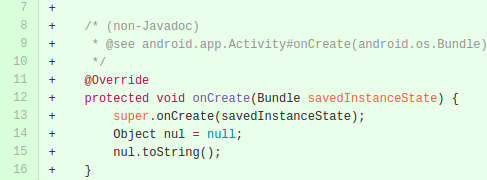
\includegraphics[width=0.80\textwidth]{images/added_example}
    \caption{Newly added method}
    \label{fig:added_method}
\end{figure}

\begin{figure}[!ht]
    \centering
        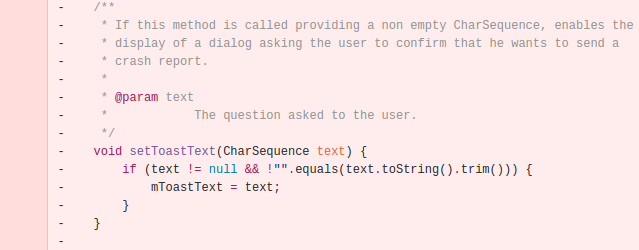
\includegraphics[width=0.80\textwidth]{images/deleted_method}
    \caption{Removed method}
    \label{fig:removed_method}
\end{figure}

\begin{figure}[!ht]
    \centering
        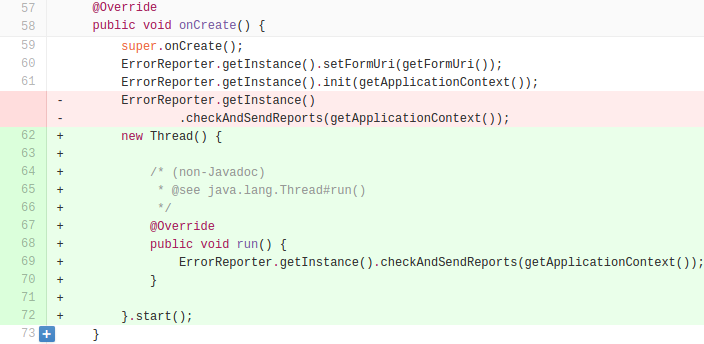
\includegraphics[width=0.80\textwidth]{images/simple_complex}
    \caption{Mixed changed method}
    \label{fig:changed_method}
\end{figure}

\begin{figure}[!ht]
    \centering
        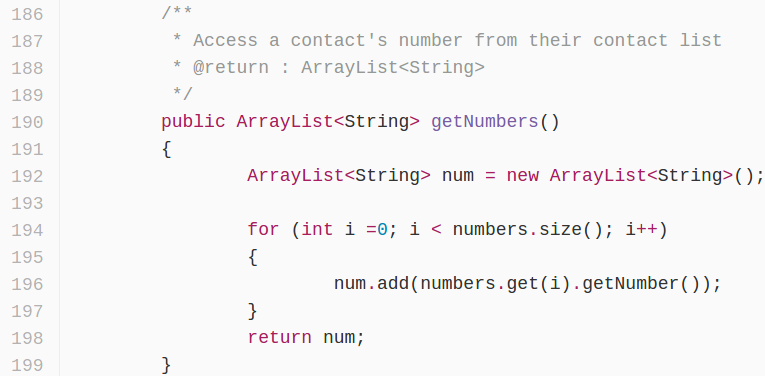
\includegraphics[width=0.80\textwidth]{images/unchanged_example}
    \caption{Unchanged method}
    \label{fig:unchanged_method}
\end{figure}


Using the patch file a \textit{deleted} file can be reconstructed by removing all lines marked as added from the file and adding the lines marked as deleted back into their original location. This allows for both added and deleted methods to be identified by using the original file for detecting the location of added methods and the \textit{deleted} file to detect deleted methods.

%- Note that an added method is one such that every line of code within it is newly added. Likewise a deleted method is one such that every line of code in removed.

The more difficult method to identify is one which has been modified. Again use of the two files will be necessary, in this case we will identify methods from each which are not entirely additions or deletions respectively. The union of these two sets of methods will be taken to determine the number of methods that have been modified. For each commit this information is stored to allow for easier access and save time since the analysis of larger datasets can be time intensive. In order to maintain the integrity of the initial dataset this information is stored in a new database.

%- TODO also describe the collection of method line changes

%<<< TODO create a table which outlines the metrics stored >>>

\section{Analysis}
\label{sec:analysis}

\subsection{SVM Predictions}
\label{subsec:svm_prediction}
% TODO talk even more about how to pick better features.

A \gls{svm} is used to predict what type of change will occur based on a set of features provided. A feature is a data extracted from the project represented as a floating point number. In order to be useful a feature must in some way characterize the the category that it is assigned to. The feature must also not rely on the category that it belongs to in order to be calculated. For example, given a category of the method change within the next 5 commits or not, then the features must not rely on knowledge of future changes to the project. If the features fail to effectively characterize the category they are assigned to then the \gls{svm} may have poor predictions. It is also necessary for the features to independent of each other to not negatively affect the categorization.

%<<< TODO Example feature vector >>>

% \begin{table}
% \begin{center}
%     \begin{tabular}{|l l l l l l l|l|}
%         \hline
        
%         Features &  &  &  &  &  &  & Description \\
%         \hline
%         $name$ & $signature$ & $change_i$ & $committer$ & $freq_{change}$ & $change_{prev}$ & $t_\Delta$ & $change_{next\_6}$ \\
%         %0.0 & 0.1 & 0.0\\
%         \hline
%     \end{tabular}
% \end{center}
% \caption{Example Feature Vector}
% \label{tab:example_feature_vector}
% \end{table}

% TODO Format parts of this.
\gls{svm} requires all feature data be encoded as floating point numbers. For any numerical data the conversion to floating point is trivial. However, for more complex data the conversion is a little more difficult. Categorical data can be mapped into a unique vector entry per category. For example, if a feature can be 1 of 3 options: 0, 1 or 2 then it can be converted into three entries in the feature vector. Encoding the value 2 the sub-vector of the feature set would be [0, 0, 1] where 1 indicates a field that feature is present in the data for this vector, and 0 indicates the feature is not present. Data that is in the form of a string can be converted to a floating point number by assigning a unique number for each string (similar to hashing). The one downside to this method is that the numbers corresponding to each string maintain no numerical properties. In essence the data becomes categorical, such that if \textit{bob} is mapped to 1 and \textit{sally} is mapped to 2 there is no relationship between 1 and 2. Ideally, this data would then be further converted using the previously described method however if the set of possible strings is large then it may be unreasonable to convert it. For example, if there are 100 possible strings then that would add 100 new entries to a single vector.

%<<< TODO svm diagrams >>>

The categorization is used for the prediction, where each value of the category relates to a unique prediction type. For example, a simple binary categorization could simply 1 or 0 where 1 predicts the event will occur and 0 predicts that the event will not occur. In essence an \gls{svm} is tasked with separating a dataset into two different categories given a sample set of data that has already been categorized into two subsets. Given the categorization of the sample dataset the \gls{svm} model is trained to allow for categorization of new data. The categorization of any new vectors (that were not used for training) is called a prediction and is made by the \gls{svm} model created through the training. More specifically, the sample dataset is a dataset extracted from the target dataset. The sample dataset is then categorized based on the predetermined criteria (the prediction goal). This dataset along with the categorization for each vector in the dataset is the training dataset, and is then used to \textit{train} the \gls{svm} model. Once the model has been trained, the \gls{svm} model is ready to be used for making classification predictions. The data for each feature can be extracted from the new dataset, allowing for the model to classify each new vector. Given that the \gls{svm} model is accurate and reliable the results can then be used towards making predictions about the dataset. For example if the classification is that of predicting change to occur within the next six commits the developer may wish to be careful with the use of the method or assess the method's quality and determine if any issues within the method need to be addressed.

A lower prediction score often relates to the data from the feature set poorly characterizing the categories. Similarly a warning will be given if the dataset is in-separate. In this case, the dataset for each category may be too similar and cannot be properly split into the two category subsets. In both cases a change to the feature set may help, whether that is a decrease or increase of features in the set. Some features are detrimental to the model, especially two features related to one another. Other potential steps would be to modify the data to ...
% *** TODO determine best practices for data something like mean of 1 and std of 1. ***

More details about the specific features used will be given a little later on. Features are descriptive aspects of the dataset that are classified into the predetermined categories. Since these features relate directly to the category understanding of the classification critical and can help determine which features should be used. For example for a classification of whether a change will occur within the next few commits, a useful feature may be the frequency by which a method changes within the project. Picking a descriptive feature set is paramount to providing a strong prediction of future data.

%<<< TODO create a figure to outline the various features and their meaning >>>

Most of this was done using database queries or user defined functions created in the database language.

\subsection{Random Forest Predictions}
\label{sec:random_forest_predictions}

Another machine learning technique investigated was \gls{rf}s. A \gls{rf} leverages numerous decision trees to provide attempt to improve prediction capabilities. Therefore to fully understand a \gls{rf} first an understanding of decision trees is necessary. A decision tree is a technique which will create a tree based on a data set that has been classified. Once the decision tree model is created it can be used to predict or categorize data that has not yet to be classified. In the tree model the leafs will be categorizations where as the connections between inner nodes are the decisions by which the categorizations are made.

One issue with decisions trees and more generally machine learning techniques in general is unbalanced data sets for training the model. The data set used rarely provided even sample sizes of each set therefore without taking necessary pro-cautions the algorithm will bias the results. In the worse case the model will classify any input data as the larger data classification.

In case of unbalanced datasets there are several methods to help provide stronger predictions. The most obvious and easiest to attempt would be to sample more data. However if the dataset in general follows this trend then some more advanced techniques can used to improve the model.

% Note when remarking about model quality this refers to accuracy and recall of the model
 
The first method would be to \textit{undersample} larger category this will even out both of the categories. This will remove some of the input values within the dataset to reduce the set size. However if there are very few samples of the smaller category the performance will suffer as well. A second method of \textit{oversampling} is useful in the case were the data samples are small. The input data from the smaller category is selected to be duplicated in the set to increase the size of the set. This helpful since it will increase the size of the dataset but could lead to bias based on the data selected from the smaller dataset. The selection method for which input vectors to over or under sample can be based off on the data's statistical distribution or made by random choice. Another advantage of these over and under sampling is that they can also be used together to in the case of a large disparity between the category's set size. 

% Bootstrapping aggregation
Another method which is used to help provide more reliable predictions is \textit{Bootstrap Aggregation}. Similar to normal sampling methods it will take the initial dataset. However rather than using the dataset as is the dataset will be uniformly sampled $n$ times and repeated $m$ times to create $m$ datasets of $n$ values. These newly created datasets will then be used to train $m$ models. Finally, when attempting to categorize a new input data it will be given to every model and the prediction result will be aggregated to provide a more accurate results. For some machine learning methods such as \gls{svm} this method will improve the results and help with unbalanced datasets.

A \gls{rf} is a collection of decisions trees trained on random samples of the initial dataset. So the \gls{rf} will take an input dataset and then train $m$ decisions trees using $m$ randomly sampled sub-datasets of the initial dataset. This helps improve the model created and makes \gls{rf}s far easier to use. Another bonus of \gls{rf}s is that the importance of each feature is assessed during the training of the model. The importance outlines the quality of each feature in providing the prediction. Therefore in order to properly understand the feature importance the accuracy, precision and recall of the model should be determined by running a test dataset to determine the quality of the model.

% TODO place the visualization in a better location
\section{Visualization}

\subsection{Line Change}

After collecting an analyzing the data the key features are extracted from the collected data. In order to to better understand resulting data it was visualized. The first visualization simply showed the changes recorded on a per line basis. These changes were divided into several closely related subcategories of additions, deletions and modifications. Additions identify changes that are new and do not have a corresponding set of deleted code. Similarly deletions refers to changes that remove code without a corresponding set of additions. Finally modifications are a set of changes which contain a set of additions and deletions that are related.

In a modification the changes are related through the \gls{ld} calculation. This distance calculation will determine the edit distance between two strings. Where edit distance is defined as the number of characters difference between two different strings. For example, \gls{ld} between \textit{happy} and \textit{mapper} would be 3, since h would be changed to m, y to e and r would be added at the end. While this provides a good initial method for comparison between two string values the value must be normalized to allow for more general use. To calculate \gls{nld} the \gls{ld} would be divided by the larger of the two strings sizes shown in equation \ref{eq:normalized_ld}.

% TODO note that a_i is an addition line and that d_j is a deletion line
% TODO clarify change block with picture

\begin{equation}
\label{eq:normalized_ld}
NLD(a_i, d_j) = \frac{LD(a_i, d_j)}{\max(|a_i|,|d_j|)}
\end{equation}

% TODO show distance calculation and paper cite this.
Modifications were assumed to only take place in a series of changes that involved both additions and deletions shown in figure \ref{fig:changed_method} and with an \gls{nld} below a defined threshold $\Delta_m$.

\begin{equation}
\label{eq:similarity_threshold}
m(a_i, d_j) = NLD(a_i, d_j) < \Delta_m
\end{equation}

In order to account for larger method signatures a threshold $\alpha$ was created to separate small and large method signatures. Therefore the equation \ref{eq:similarity_threshold} was updated accordingly shown in equation \ref{eq:complete_similarity_threshold}.

\begin{equation}
\label{eq:complete_similarity_threshold}
m(a_i, d_j) = \left\{\begin{matrix}
NLD(a_i, d_j) < \Delta_s & \text{if } \max(|a_i|, |d_j|) < \alpha \\ 
NLD(a_i, d_j) < \Delta_l & \text{otherwise}
\end{matrix}\right.
\end{equation}

Lines that are part of the same block of additions and deletions are selected for the similarity check to determine whether they can be classified as a modification. Modifications will consist of one to many addition lines mapped to one to many lines of deletion. Therefore a modification is more easily referred to as a modification set.

For addition lines that do not meet the threshold of similarity with any deletion line in the change block are classified as additions. Similarly, deletion lines who fail to meet the similarity threshold for any addition lines will be classified as deletions. Therefore a block of changes will contain a set of additions, deletions and modifications any of which may be empty.

% TODO talk about comments.

% TODO talk about the summary stats

% Discuss the slight controls that each one allows and the special one just for this view. TODO place this better.
The project's tags are shown at the bottom of each graph optionally to potentially provide some context. Since these tags often mark points of significant within the project they can be thought as road signs. The site also provides some options to refine or generalize the graphs. For all of the graphs you are allowed to select the project, package path, and the committers you wish to view. Specifically for the line level graph a further option is provided to condense the data based on a monthly, weekly summary.

% TODO fit in the commit information shown
As a further guide marker the commit information is provided (when viewing either line at the commit view, method level or statement level). This information allows for a direct link to the project and can be a handy tool for referring back to the software repository.

% TODO sample image of visualization

\subsection{Method Change}

The visualization of line changes was very noisy and proved difficult to use. Instead of viewing every line of change separately they were grouped together based on the method from which they originate from. Similar classifications are used for method changes however their definitions vary slightly. There are three types of method level changes that can occur. Firstly, a method can be newly added implying that the method had not existed in the previous version. Secondly, a deleted method implying that the method is completely removed from the current version. Thirdly, a method can be modified by containing a set of changes that are not constituting the entire method changing. 
% TODO show example of each.

It should be noted that at the method level comment changes are ignored. Instead the focus is placed on that of the three types of changes. The visualization for the method level uses a bar graph since it provided a more clear picture of the relationship between commits. Rather than as the first visualization did imply that a relationship was to be drawn between different commits of the same type only changes of the same time are grouped together. The contrast in magnitude between each type of change and each commit is also more clear and defines the visualization.

% TODO show image

\subsection{Method Statement Change}

The method level visualization provided a fairly clear higher level view of the data. However, while collecting that data lower level data was collected as part of the previous analysis. This afforded a combination of the previous two methods. While more data is available and is quite overwhelming the final graph could provide some use when used in conjunction with the previous graph.

The view itself classifies changes into several categories, first their is \textit{Added} changes which comes in the form of both code and comments. Secondly, \textit{Deleted} changes which again is for both code and comments. Similar to that of the method level added or deleted method these statements belong to methods that are either entirely added or deleted from the project. However for this level each statement is counted versus just the method on whole.

The more complicated categories are introduced as part of the modification classifications. These all stem from the method level modifications. A modified method will contain some changes which can be statement additions or deletions. Therefore modifications are divided into modifications that are additions and ones that are deletions. The final filter is again based on statements being either comments are code. So finally we have the categories: \textit{Modified Code Added}, \textit{Modified Comment Added}, \textit{Modified Code Deleted} and \textit{Modified Comment Deleted}.

% TODO show image

% Decided whether to keep the other names or update them to these ones (on the site as well).
%So finally we have the categories: \textit{Modified Code Addition}, \textit{Modified Comment Addition}, \textit{Modified Code Deletion} and \textit{Modified Comment Deletion}.